% Provenance (never printed): see sources/outline_sources.md (Year 1: compaction and
% cementation; basin types; subsidence, accommodation and sea-level change). Exercise and
% problem values in the Book 3 scratch calculator calc/ch23.py; figure data from
% figdata/bachelor-1/compaction.py and sea_level.py.
% Porosity and permeability are Book 1's (g6); diagenesis was met in Book 2 (g12) and is
% re-founded here; sedimentary basin was met in Book 2 (g11) and is re-founded here;
% isostasy and the equal-mass proposition are ch. 11's; passive margins and rifts ch. 13's;
% effective stress ch. 16's; the Last Glacial Maximum and glacial cycles Book 2's (g12).
% Pressure solution is defined in the Year 3 volume (deformation mechanisms): prose only.
% Backstripping, the stretching model and the comparison of basins are the Year 2 volume's.
\chapter{Diagênese e bacias sedimentares}\label{ch:b1:diagenesis-basins}

A areia de praia é solta: metade dela, em volume, é água entre os grãos. Soterrada a três
quilômetros de profundidade, a mesma areia volta em um testemunho de sondagem como arenito
duro, seus grãos comprimidos uns contra os outros e o espaço entre eles muito reduzido e
em parte preenchido por quartzo novo. Entre a praia e o testemunho há milhões de anos em
que o sedimento foi soterrado sob mais sedimento, comprimido, aquecido e embebido em água
que dissolveu alguns \omterm{def:b1:rock-forming-minerals:mineral}{minerais} e depositou outros. Este capítulo acompanha essas mudanças e
depois dá um passo atrás, até os lugares onde o sedimento pode se acumular em quilômetros de
espessura (as \omterm{def:b1:diagenesis-basins:basin}{bacias sedimentares}) e até as duas coisas que lhes abrem espaço: o afundamento
do fundo e a subida e a descida do mar.

\begin{recall}
A porosidade de uma rocha é a fração de seu volume formada por poros, e sua permeabilidade
mede quão facilmente a água flui através deles (Livro~1, 6º ano). Uma região está em
\omterm{def:b1:isostasy-gravity:isostasy}{isostasia} quando toda coluna até a \omterm{def:b1:isostasy-gravity:isostasy}{profundidade de compensação} contém a mesma massa
(\cref{prop:b1:isostasy-gravity:equal-mass}). Riftes se abrem por falhas normais, e margens
passivas são as bordas dos continentes deixadas para trás quando um rifte se torna oceano
(\cref{ch:b1:rifts-ridges-margins}). A \omterm{def:b1:stress-strain-rheology:lithostatic}{tensão efetiva} é a tensão menos a \omterm{def:b1:stress-strain-rheology:lithostatic}{pressão do fluido
nos poros} (\cref{def:b1:stress-strain-rheology:lithostatic}). O último ciclo glacial atingiu
seu Último Máximo Glacial há cerca de vinte mil anos (Livro~2, 12º ano). Arenitos, folhelhos
e seus ambientes são os de \cref{ch:b1:clastic-sediments}; calcários, giz, dolomita e
\omterm{def:b1:chemical-biogenic-sediments:evaporite}{evaporitos} são os de \cref{ch:b1:chemical-biogenic-sediments}.
\end{recall}

\section{Compactação}\label{sec:b1:diagenesis-basins:compaction}

Um sedimento recém-depositado é um empacotamento solto de grãos com água entre eles. Tudo o
que acontece com ele depois da deposição e antes do metamorfismo, enquanto permanece nas
baixas temperaturas e pressões dos poucos quilômetros superiores da \omterm{def:b1:layered-earth:layers}{crosta}, pertence a uma
só família de processos.

\begin{definition}[Diagênese]\label{def:b1:diagenesis-basins:diagenesis}
\emph{Diagênese}\index{diagênese} é o conjunto de mudanças físicas, químicas e biológicas
que um sedimento sofre após sua deposição, nas temperaturas e pressões da \omterm{def:b1:layered-earth:layers}{crosta} superior,
abaixo das do metamorfismo. Inclui a \omterm{def:b1:diagenesis-basins:compaction}{compactação}, a \omterm{def:b1:diagenesis-basins:cement}{cimentação}, a dissolução de grãos e a
substituição de um \omterm{def:b1:rock-forming-minerals:mineral}{mineral} por outro; juntas, elas transformam um sedimento solto em uma
rocha sedimentar.
\end{definition}

A primeira dessas mudanças é mecânica. Cada nova camada soma seu peso ao das que estão
abaixo. Os grãos são comprimidos, deslizam e giram para um empacotamento mais apertado, os
moles (lamelas de argila, fragmentos de rocha, \omterm{def:b1:rock-forming-minerals:groups}{micas}) se dobram entre os duros, e a água
entre eles é expulsa.
% ledger: og:diagenesis

\begin{definition}[Compactação, descompactação]\label{def:b1:diagenesis-basins:compaction}
\emph{Compactação}\index{compactação} é a perda de volume de um sedimento sob o peso dos
sedimentos acima dele, pelo empacotamento mais fechado de seus grãos, pela expulsão de sua
água de poros e, mais fundo, pela dissolução de grãos onde se tocam.
\emph{Descompactação}\index{descompactação} é o cálculo que restitui uma camada soterrada à
espessura que tinha em um soterramento anterior, mais raso, mais frequentemente na
superfície, quando foi depositada.
\end{definition}

As porosidades medidas em poços caem com a profundidade, bruscamente perto da superfície e
depois cada vez mais devagar. Em 1930, L.~F. Athy ajustou-as com uma exponencial, e o ajuste
tem sido o ponto de partida dos estudos de \omterm{def:b1:diagenesis-basins:compaction}{compactação} desde então.
% ledger: sc80:athy

\begin{proposition}[Lei de Athy]\label{prop:b1:diagenesis-basins:athy}
Em uma pilha de sedimento de uma só litologia, compactada sob o próprio peso com a água de
poros livre para escapar, a porosidade à profundidade $z$ abaixo da superfície é
\[
  \varphi(z) = \varphi_0\, e^{-z/\lambda},
\]
em que $\varphi_0$, a porosidade superficial, e $\lambda$, o comprimento de decaimento,
dependem da litologia. Esta é a \emph{lei de Athy}\index{lei de Athy}.
\end{proposition}
\admitted

A lei é um ajuste empírico, não uma consequência da teoria. Seus parâmetros são medidos,
litologia por litologia, a partir das porosidades de poços; os valores da
\cref{tab:b1:diagenesis-basins:athy}, publicados com um estudo do afundamento do Mar do
Norte, são muito usados para corrigir a \omterm{def:b1:diagenesis-basins:compaction}{compactação}. O folhelho começa com mais água que a
areia, mas a perde em uma distância menor; o giz, o mais poroso dos três na superfície, a
perde mais depressa de todos. A \qty{3000}{m} a lei dá uma porosidade de \num{0.22} para o
arenito, \num{0.14} para o folhelho e \num{0.08} para o giz (figura abaixo): a areia de praia da
abertura do capítulo perdeu mais da metade de seus poros.
% ledger: pybacktrack:compaction, sc80:north-sea

\begin{table}[htbp]
\centering
\begin{tabular}{lccc}
\hline
litologia & porosidade superficial $\varphi_0$ & decaimento $\lambda$ (m) & densidade do grão (\unit{kg.m^{-3}}) \\
\hline
folhelho         & 0.63 & 1960 & 2700 \\
arenito          & 0.49 & 3704 & 2650 \\
arenito argiloso & 0.56 & 2564 & 2680 \\
giz              & 0.70 & 1408 & 2710 \\
\hline
\end{tabular}
\caption{Os parâmetros da \omterm{prop:b1:diagenesis-basins:athy}{lei de Athy} e as densidades dos grãos para quatro litologias,
segundo Sclater e Christie (1980), como tabulados no software aberto de retrodescompactação
pyBacktrack.}
\label{tab:b1:diagenesis-basins:athy}
\end{table}
% ledger: pybacktrack:compaction

A \omterm{def:b1:diagenesis-basins:compaction}{compactação} espreme a água; ela não acrescenta grãos nem os retira, desde que nada seja
dissolvido e levado embora ou trazido como \omterm{def:b1:diagenesis-basins:cement}{cimento}. O volume dos grãos em uma coluna é,
portanto, a quantidade a seguir à medida que a coluna é soterrada.

\begin{proposition}[Espessura sólida de uma camada]\label{prop:b1:diagenesis-basins:solid}
Sob a \omterm{prop:b1:diagenesis-basins:athy}{lei de Athy}, uma camada entre as profundidades $z_1 < z_2$ contém, por unidade de
área, um volume de grãos igual à espessura
\[
  s = (z_2 - z_1) - \varphi_0 \lambda \left( e^{-z_1/\lambda} - e^{-z_2/\lambda} \right).
\]
Se a camada for movida a uma nova profundidade sem perda ou ganho de grãos, seu novo topo
$z_1'$ e fundo $z_2'$ satisfazem $s(z_1', z_2') = s(z_1, z_2)$, e para um dado $z_1'$ essa
equação tem exatamente uma solução $z_2'$.
\end{proposition}

\begin{proof}
Uma fatia de espessura $\mathrm dz$ à profundidade $z$ contém o volume de grãos
$(1 - \varphi(z))\,\mathrm dz$ por unidade de área. Integrando de $z_1$ a $z_2$,
\[
  s = \int_{z_1}^{z_2} \bigl(1 - \varphi_0 e^{-z/\lambda}\bigr)\,\mathrm dz
    = (z_2 - z_1) - \varphi_0\lambda\left(e^{-z_1/\lambda} - e^{-z_2/\lambda}\right).
\]
Com o topo fixo em $z_1'$, a função $f(b) = s(z_1', b)$ tem a derivada $1 - \varphi(b) > 0$,
pois uma porosidade é menor que um; ela é contínua, nula em $b = z_1'$ e cresce sem limite,
de modo que assume o valor $s(z_1, z_2)$ exatamente uma vez.
\end{proof}

\begin{method}[Descompactando uma camada]\label{met:b1:diagenesis-basins:decompaction}
\begin{enumerate}
  \item Leia o topo $z_1$ e a base $z_2$ da camada hoje, e seus parâmetros $\varphi_0$ e
        $\lambda$
        (\cref{tab:b1:diagenesis-basins:athy}).
  \item Calcule sua espessura sólida $s$ com
        \cref{prop:b1:diagenesis-basins:solid}.
  \item Escolha a profundidade $z_1'$ de seu topo no tempo anterior --- zero para
        restituí-la à superfície.
  \item Resolva $s(z_1', b) = s$ para a nova base $b$ pelo método de Newton: comece com
        $b_0 = z_1' + (z_2 - z_1)$ e repita
        \[
          b_{k+1} = b_k - \frac{s(z_1', b_k) - s}{1 - \varphi(b_k)}
        \]
        até que a variação seja menor que a precisão desejada; duas ou três etapas costumam
        bastar.
  \item A espessura da camada nesse tempo é $b - z_1'$; sua porosidade média é
        $1 - s/(b - z_1')$.
\end{enumerate}
\end{method}

Tome \qty{500}{m} de folhelho entre \qty{3000}{m} e \qty{3500}{m}. Ele contém \qty{440}{m}
de grãos e apenas \qty{60}{m} de água, uma porosidade média de \num{0.12}. Trazidos de volta
à superfície, os mesmos grãos formam uma camada de \qty{891}{m} de espessura, metade dela
água (figura abaixo). A espessura de um folhelho soterrado é pouco mais da metade do que foi
depositado; taxas de sedimentação lidas em seções soterradas devem ser descompactadas antes
de serem comparadas com taxas medidas hoje.
% computed in figdata/bachelor-1/compaction.py; ledger: pybacktrack:compaction

\begin{omfigure}
\begin{tikzpicture}[font=\footnotesize]
\begin{axis}[name=phi, width=7.6cm, height=7.2cm, xmin=0, xmax=0.75, ymin=0, ymax=5000,
    y dir=reverse, xlabel={porosidade $\varphi$}, ylabel={profundidade (m)},
    xtick={0,0.2,0.4,0.6}, ytick={0,1000,...,5000},
    legend style={at={(0.97,0.03)}, anchor=south east, font=\scriptsize, draw=none, fill=white, fill opacity=0.85, text opacity=1},
    legend cell align=left]
  \addplot[thick, omLithSand!50!black] table[x=phi_sand, y=z] {figdata/out/bachelor-1-compaction-curves.dat};
  \addplot[thick, omThm, densely dashed] table[x=phi_shale, y=z] {figdata/out/bachelor-1-compaction-curves.dat};
  \addplot[thick, omLithLime!50!black, dash dot] table[x=phi_chalk, y=z] {figdata/out/bachelor-1-compaction-curves.dat};
  \legend{arenito, folhelho, giz}
  \draw[black!50, dotted] (axis cs:0,3000) -- (axis cs:0.75,3000);
\end{axis}
\begin{axis}[at={(phi.east)}, anchor=west, xshift=1.6cm, width=6.4cm, height=7.2cm,
    ybar stacked, bar width=1.1cm, ymin=0, ymax=1000, enlarge x limits=0.45,
    symbolic x coords={buried, surface}, xtick=data,
    xticklabels={{a 3000--3500 m}, {na superfície}},
    ylabel={espessura da camada (m)}, ytick={0,200,...,1000},
    legend style={at={(0.03,0.97)}, anchor=north west, font=\scriptsize, draw=none},
    legend cell align=left]
  \addplot[fill=omLithShale, draw=black!60] table[x=state, y=solid] {figdata/out/bachelor-1-compaction-demo.dat};
  \addplot[fill=omSea, draw=black!60] table[x=state, y=pore] {figdata/out/bachelor-1-compaction-demo.dat};
  \legend{grãos, água de poros}
  \node[anchor=south] at (axis cs:buried,500) {\qty{500}{m}};
  \node[anchor=south] at (axis cs:surface,891) {\qty{891}{m}};
\end{axis}
\end{tikzpicture}

{\small À esquerda: porosidade em função da profundidade pela \omterm{prop:b1:diagenesis-basins:athy}{lei de Athy} para arenito,
folhelho e giz, com os parâmetros da \cref{tab:b1:diagenesis-basins:athy}. À direita:
\qty{500}{m} de folhelho entre \qty{3000}{m} e \qty{3500}{m}, e a mesma camada descompactada
até a superfície: os grãos (\qty{440}{m}) são mantidos, a água não.}
\label{fig:b1:diagenesis-basins:compaction}
\end{omfigure}
% computed in figdata/bachelor-1/compaction.py; ledger: pybacktrack:compaction

A \omterm{prop:b1:diagenesis-basins:athy}{lei de Athy} vale apenas enquanto a água puder sair. A \omterm{def:b1:diagenesis-basins:compaction}{compactação} é impulsionada pela
\omterm{def:b1:stress-strain-rheology:lithostatic}{tensão efetiva}, o peso da rocha acima menos a pressão da água nos poros
(\cref{ch:b1:stress-strain-rheology}). Onde um folhelho espesso é soterrado mais depressa do
que sua água consegue escapar, a água carrega parte da carga, a pressão nos poros sobe acima
da hidrostática, e o folhelho mantém uma porosidade alta demais para sua profundidade: ele
está sobrepressurizado, e a correção para a \omterm{def:b1:diagenesis-basins:compaction}{compactação} deve levar isso em conta.
% ledger: sc80:north-sea

Mais fundo, a \omterm{def:b1:diagenesis-basins:compaction}{compactação} torna-se química. Onde dois grãos de quartzo se pressionam um
contra o outro através de uma película de água, e sobretudo onde uma lamela de argila ou
\omterm{def:b1:rock-forming-minerals:groups}{mica} fica entre eles, o quartzo se dissolve no contato; a sílica difunde-se um pouco através
da água e é depositada de novo em superfícies limpas de quartzo voltadas para os poros
abertos. Os grãos se interpenetram, e a dissolução concentrada ao longo das superfícies deixa
estilólitos, veios serrilhados do resíduo insolúvel. Esta dissolução por pressão, que o
Livro~5 trata como um mecanismo de deformação, é ao mesmo tempo o último estágio da
\omterm{def:b1:diagenesis-basins:compaction}{compactação} e a fonte do \omterm{def:b1:diagenesis-basins:cement}{cimento} mais comum dos arenitos.
% ledger: walderhaug:quartz, oye:quartz-cement

\section{Cimentação e outras alterações}\label{sec:b1:diagenesis-basins:cementation}

A \omterm{def:b1:diagenesis-basins:compaction}{compactação} sozinha produz um sedimento denso, não uma rocha dura. Os grãos são colados
em uma rocha por \omterm{def:b1:rock-forming-minerals:mineral}{minerais} que crescem nos poros.

\begin{definition}[Cimentação, cimento]\label{def:b1:diagenesis-basins:cement}
\emph{Cimentação}\index{cimentação} é a precipitação de \omterm{def:b1:rock-forming-minerals:mineral}{minerais} da água de poros nos poros
de um sedimento, o que une seus grãos e reduz sua porosidade. Os \omterm{def:b1:rock-forming-minerals:mineral}{minerais} assim
precipitados formam o \emph{cimento}\index{cimento} da rocha; os mais comuns são quartzo,
calcita, óxidos de ferro e \omterm{def:b1:rock-forming-minerals:mineral}{minerais} de argila.
\end{definition}

A água subterrânea carrega os \omterm{def:b1:rock-forming-minerals:mineral}{minerais} cimentantes em solução, e eles não precisam ter a
mesma composição dos grãos. Óxidos de ferro revestem os grãos e colorem as rochas de
vermelho, marrom ou amarelo, como nas camadas do Planalto do Colorado; a calcita cimenta
arenitos e calcários igualmente.
% ledger: og:diagenesis

O quartzo é o \omterm{def:b1:diagenesis-basins:cement}{cimento} de arenitos profundamente soterrados. Ele cresce sobre os grãos
detríticos de quartzo em continuidade óptica com eles, como sobrecrescimentos: ao microscópio,
um grão e seu sobrecrescimento escurecem juntos entre \omterm{def:b1:field-lab-methods-1:microscope}{polarizadores cruzados}, e o contorno
original do grão aparece apenas como uma fina borda de pó ou argila (figura abaixo). Em
arenitos do Mar do Norte e do Texas estudados em detalhe, os isótopos de oxigênio dos
sobrecrescimentos mostram que o \omterm{def:b1:diagenesis-basins:cement}{cimento} começou a crescer a \qtyrange{60}{80}{\celsius} e
continuou até as rochas atingirem sua maior temperatura de soterramento; os arenitos do Texas
contêm \qtyrange{12}{18}{\percent} de \omterm{def:b1:diagenesis-basins:cement}{cimento} de quartzo, os do Mar do Norte apenas
\qtyrange{2}{6}{\percent}, e a maior parte da sílica veio da dissolução por pressão nos \omterm{def:b1:geological-maps:geological-map}{contatos}
entre grãos. Como o quartzo cresce apenas em superfícies limpas de quartzo, um revestimento
de argila sobre os grãos deixa menos superfície para o \omterm{def:b1:diagenesis-basins:cement}{cimento} e pode preservar a porosidade
de um arenito profundo.
% ledger: oye:quartz-cement, walderhaug:quartz

\begin{omfigure}
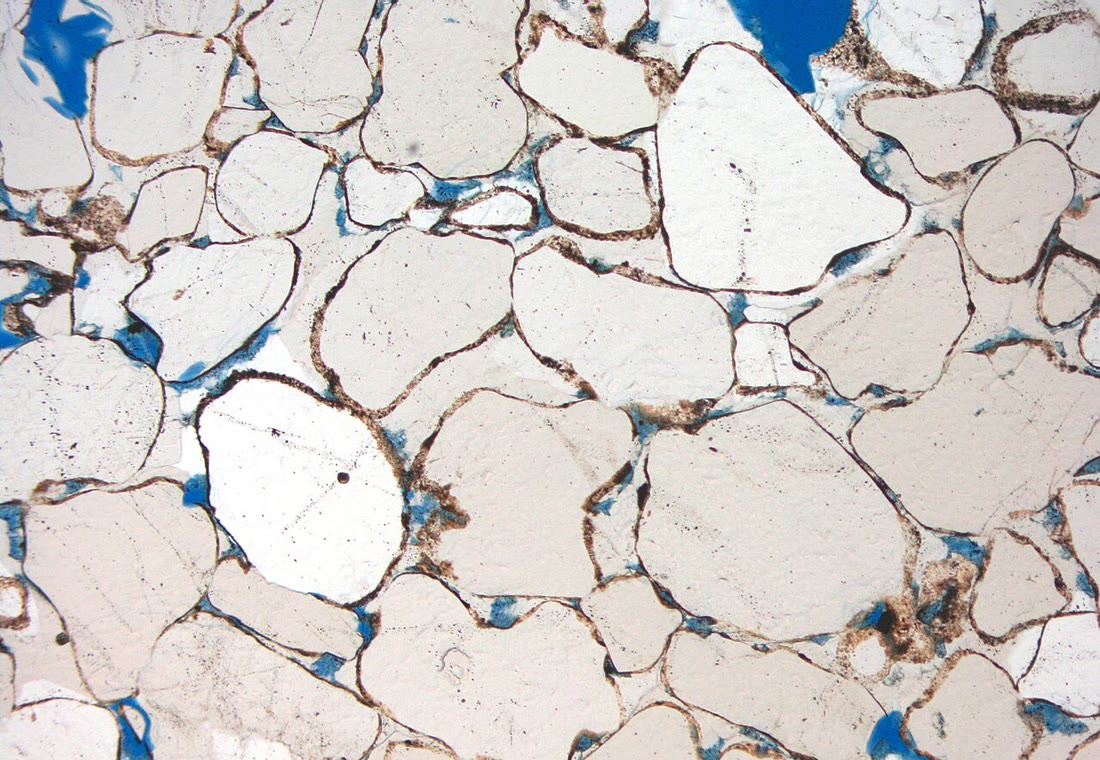
\includegraphics[width=0.62\linewidth]{images/book3/b1-quartz-overgrowths.jpg}

{\small Uma \omterm{def:b1:field-lab-methods-1:thin-section}{lâmina delgada} de arenito de quartzo, o Arenito de Potsdam (Cambriano) do estado
de Nova York, em luz polarizada plana. Os grãos detríticos arredondados são delineados por
bordas escuras de pó e argila; o quartzo claro fora dessas bordas é \omterm{def:b1:diagenesis-basins:cement}{cimento} que cresceu sobre
os grãos, em continuidade óptica com eles, até que os sobrecrescimentos vizinhos se
encontrassem em faces retas. Resina azul preenche o que resta dos poros. (M.~C.~Rygel,
CC~BY-SA~4.0, via Wikimedia Commons; barra de escala do original cortada.)}
\label{fig:b1:diagenesis-basins:overgrowths}
\end{omfigure}
% ledger: commons:potsdam

Nem toda mudança destrói porosidade. Água subsaturada em um \omterm{def:b1:rock-forming-minerals:mineral}{mineral} o dissolve: grãos de
\omterm{def:b1:rock-forming-minerals:groups}{feldspato} e de carbonato, e \omterm{def:b1:diagenesis-basins:cement}{cimentos} carbonáticos anteriores, podem ser removidos e deixar
uma porosidade secundária, poros com a forma dos grãos que substituem. \omterm{def:b1:rock-forming-minerals:mineral}{Minerais} de argila
crescem nos poros por sua vez, como revestimentos sobre os grãos ou como cristais que
preenchem os poros e estreitam as passagens entre eles, reduzindo a permeabilidade. Os
\omterm{def:b1:rock-forming-minerals:mineral}{minerais} do sedimento também mudam: a aragonita das conchas e da \omterm{def:b1:chemical-biogenic-sediments:factory}{fábrica de carbonatos} volta
a calcita, que é estável na superfície, e a calcita, na presença de água com magnésio, pode
tornar-se dolomita.
% ledger: og:diagenesis

A substituição de calcita por dolomita, a dolomitização, é uma reação com magnésio da água,
\[
  \ce{2 CaCO3 + Mg^2+ -> CaMg(CO3)2 + Ca^2+},
\]
e ela muda o volume do sólido.

\begin{proposition}[Dolomitização cria porosidade]\label{prop:b1:diagenesis-basins:dolomite}
Se dois mols de calcita de densidade $\rho_c$ são substituídos por um mol de dolomita de
densidade $\rho_d$, o volume do sólido diminui na fração
\[
  1 - \frac{M_d/\rho_d}{2M_c/\rho_c},
\]
onde $M_c$ e $M_d$ são as massas molares. Com $\rho_c = \qty{2.71}{g.cm^{-3}}$ e
$\rho_d = \qty{2.84}{g.cm^{-3}}$ essa fração é \qty{12.1}{\percent}.
\end{proposition}

\begin{proof}
O volume molar de um \omterm{def:b1:rock-forming-minerals:mineral}{mineral} é sua massa molar dividida por sua densidade. Dois mols de
calcita ocupam $2M_c/\rho_c$ e um de dolomita $M_d/\rho_d$; a fração perdida é um menos a
razão entre eles. Com $M_c = \qty{100.09}{g.mol^{-1}}$ e $M_d = \qty{184.40}{g.mol^{-1}}$ os
dois volumes são $2\times\qty{36.93}{cm^3} = \qty{73.86}{cm^3}$ e \qty{64.93}{cm^3}, e
$1 - 64.93/73.86 = \num{0.121}$.
\end{proof}

Se o volume externo da rocha não muda, o sólido perdido é espaço de poros ganho: um calcário
de porosidade \num{0.10} substituído mol por mol por dolomita tem porosidade de cerca de
\num{0.21}. A reação precisa de muito magnésio, que a água do mar contém cerca de
\qty{1.28}{g} por quilograma; ela é favorecida onde salmouras ou água do mar fluem pela rocha
por muito tempo (\cref{exo:b1:diagenesis-basins:12}).
% ledger: hom:calcite, webmineral:others, teos10:reference-composition, teos10:reference-salinity

A \omterm{def:b1:diagenesis-basins:diagenesis}{diagênese} segue a história do sedimento. Logo após a deposição, perto da superfície, a
água de poros ainda é a do mar, do lago ou da chuva: os sedimentos são bioturbados,
cimentados cedo no fundo do mar ou no solo, e a aragonita se transforma em calcita. Com o
soterramento e o aquecimento, dominam a \omterm{def:b1:diagenesis-basins:compaction}{compactação}, a dissolução por pressão e o \omterm{def:b1:diagenesis-basins:cement}{cimento}
de quartzo. Se a bacia for depois soerguida e erodida, água doce da superfície volta às
rochas e dissolve de novo carbonato e \omterm{def:b1:rock-forming-minerals:groups}{feldspato}. Uma \omterm{def:b1:field-lab-methods-1:thin-section}{lâmina delgada} registra a ordem desses
eventos: um \omterm{def:b1:diagenesis-basins:cement}{cimento} que preenche o poro deixado por um grão dissolvido é mais jovem que a
dissolução, e um sobrecrescimento quebrado pela \omterm{def:b1:diagenesis-basins:compaction}{compactação} é mais antigo que a \omterm{def:b1:diagenesis-basins:compaction}{compactação}.

\section{Bacias sedimentares}\label{sec:b1:diagenesis-basins:basins}

Sedimento com quilômetros de espessura só se acumula onde o fundo continua afundando.

\begin{definition}[Bacia sedimentar]\label{def:b1:diagenesis-basins:basin}
Uma \emph{bacia sedimentar}\index{bacia sedimentar} é uma região da superfície da Terra onde a
\omterm{def:b1:layered-earth:layers}{crosta} afundou por muito tempo, de alguns milhões a algumas centenas de milhões de anos, e
onde o espaço assim criado foi preenchido por sedimento, de centenas de metros a muitos
quilômetros de espessura.
\end{definition}

\begin{definition}[Subsidência, subsidência tectônica]\label{def:b1:diagenesis-basins:subsidence}
A \emph{subsidência}\index{subsidência} de uma bacia é o movimento para baixo de seu
embasamento, a superfície sobre a qual repousam seus sedimentos, medido em relação a uma
referência fixa, como o centro da Terra. Sua \emph{subsidência tectônica}\index{subsidência tectônica} é a parte devida aos processos que formam a bacia, distinta do afundamento extra
causado pelo peso dos sedimentos e da água que a preenchem; ela é medida pela subsidência que
o embasamento teria tido sob a água apenas.
\end{definition}

O que faz o fundo afundar é a posição da bacia na placa (figura abaixo).

\begin{description}
  \item[Bacias de rifte.] Falhas normais estiram a \omterm{def:b1:layered-earth:layers}{crosta}, e blocos afundam entre elas
        (\cref{ch:b1:rifts-ridges-margins}). As bacias são estreitas e assimétricas, \omterm{def:b1:rifts-ridges-margins:rift}{meio-grábens}
        preenchidos mais depressa contra sua falha de borda. Os campos petrolíferos do Mar do
        Norte situam-se nas estruturas de seus \omterm{def:b1:rifts-ridges-margins:rift}{grábens} de Viking e Central, soterrados sob
        sedimentos mais jovens. Quando o estiramento para, a \omterm{def:b1:layered-earth:lithosphere}{litosfera} afinada e aquecida
        esfria, contrai-se e continua afundando, devagar, por dezenas de milhões de anos. O
        Mar do Norte central, cujo último estiramento importante terminou no meio do Cretáceo,
        afundou então como uma bacia larga em forma de pires, preenchida sucessivamente por giz,
        arenitos e, durante a maior parte do Terciário, folhelhos e lamitos; seu embasamento,
        carregado só pela água, teria afundado \qtyrange{1100}{1400}{m} no centro.
  \item[Margens passivas.] Quando o rifte se torna oceano, o mesmo resfriamento faz cada
        margem afundar após a separação, e uma cunha de sedimento que engrossa em direção ao
        oceano se acumula sobre as antigas bacias de rifte.
  \item[Bacias de antepaís.] Diante de um cinturão de cavalgamentos, o peso das escamas
        empilhadas dobra a \omterm{def:b1:layered-earth:lithosphere}{litosfera} para baixo, por \omterm{def:b1:isostasy-gravity:isostasy}{isostasia}, formando uma bacia mais funda
        junto ao cinturão e preenchida pelos detritos erodidos dele. A maior parte das rochas
        cretáceas do oeste do Canadá foi depositada em uma bacia assim, diante das Montanhas
        Rochosas.
  \item[Bacias intracratônicas.] No interior de continentes antigos, longe de qualquer limite
        de placa, regiões amplas, redondas ou ovais afundaram devagar por tempos muito longos.
        A Bacia de Paris é o centro de uma depressão estrutural assim, entre os antigos maciços
        da Bretanha, do Maciço Central e dos Vosges e Ardenas.
  \item[Bacias de \omterm{def:b1:faults-folds-fabrics:fault-types}{falha transcorrente}.] Onde uma \omterm{def:b1:faults-folds-fabrics:fault-types}{falha transcorrente} dá um passo lateral no
        sentido que afasta suas paredes --- uma curva distensiva ---, um paralelogramo de
        \omterm{def:b1:layered-earth:layers}{crosta} afunda entre os dois ramos da falha: uma bacia pull-apart, como as da região de
        Los Angeles ao longo do sistema de San Andreas.
\end{description}
% ledger: ws:basins, sc80:north-sea, britannica:paris-basin

A razão pela qual a \omterm{def:b1:layered-earth:lithosphere}{litosfera} afunda em cada cenário, com que taxa, e como as bacias se
comparam, é o assunto do Livro~4; aqui elas são distinguidas pelo lugar onde estão e pela
forma de seu preenchimento.

\begin{omfigure}
\begin{tikzpicture}[font=\scriptsize, line join=round]
% (a) rift: a half-graben
\begin{scope}
  \fill[lith granite] (0,0) -- (0,1.6) -- (1.4,1.6) -- (2.2,0.2) -- (5.0,1.0) -- (5.0,0) -- cycle;
  \fill[lith shale] (1.4,1.6) -- (2.2,0.2) -- (5.0,1.0) -- (5.0,1.6) -- cycle;
  \fill[lith sandstone] (1.4,1.6) -- (1.75,0.99) -- (5.0,1.25) -- (5.0,1.6) -- cycle;
  \draw[normal fault, thick] (1.4,1.6) -- (2.3,0.0);
  \draw[black!70] (0,1.6) -- (5.0,1.6);
  \node[anchor=south west] at (0,1.65) {(a) rifte: um meio-gráben};
  \node[fill=white, fill opacity=0.8, text opacity=1, inner sep=1pt] at (3.9,0.3) {embasamento};
  \node[fill=white, fill opacity=0.8, text opacity=1, inner sep=1pt] at (0.65,0.8) {muro};
\end{scope}
% (b) passive margin: a seaward-thickening wedge over thinned crust
\begin{scope}[xshift=6.6cm]
  \fill[lith sea] (2.0,1.6) -- (5.0,1.6) -- (5.0,0.75) -- (3.6,0.95) -- cycle;
  \fill[lith granite] (0,0) -- (0,1.2) -- (2.0,1.0) -- (3.6,0.35) -- (5.0,0.05) -- (5.0,0) -- cycle;
  \fill[lith shale] (0,1.2) -- (2.0,1.0) -- (3.6,0.35) -- (5.0,0.05) -- (5.0,0.75) -- (3.6,0.95) -- (2.0,1.6) -- (0,1.6) -- cycle;
  \draw[black!70] (0,1.6) -- (2.0,1.6) -- (3.6,0.95) -- (5.0,0.75);
  \draw[blue!60!black, thick] (2.0,1.6) -- (5.0,1.6);
  \node[anchor=south west] at (0,1.65) {(b) margem passiva};
  \node[fill=white, fill opacity=0.8, text opacity=1, inner sep=1pt] at (1.0,0.45) {crosta continental afinada};
  \node[anchor=north east] at (5.0,1.58) {oceano};
\end{scope}
% (c) foreland basin: asymmetric, deepest against the thrust belt
\begin{scope}[yshift=-3.3cm]
  \fill[lith granite] (0,0) -- (0,0.55) -- (5.0,1.35) -- (5.0,0) -- cycle;
  \fill[lith sandstone] (0,0.55) -- (5.0,1.35) -- (5.0,1.6) -- (0,1.6) -- cycle;
  \fill[lith conglomerate] (1.0,1.6) -- (3.6,1.6) -- (1.0,1.0) -- cycle;
  \fill[omLithSchist, draw=black!70] (0,0.95) -- (1.9,1.6) -- (1.3,1.95) -- (0.4,2.25) -- (0,2.3) -- cycle;
  \draw[thrust fault] (0,0.95) -- (1.9,1.6);
  \draw[thrust fault] (0,1.55) -- (1.15,1.95);
  \draw[black!70] (1.9,1.6) -- (5.0,1.6);
  \node[anchor=south west] at (2.0,1.65) {(c) bacia de antepaís};
  \node[anchor=south west, inner sep=1pt] at (0.25,2.3) {cinturão de cavalgamento};
  \node[fill=white, fill opacity=0.8, text opacity=1, inner sep=1pt] at (3.9,0.35) {embasamento};
\end{scope}
% (d) intracratonic basin: a broad sag, layers thickening to the centre
\begin{scope}[xshift=6.6cm, yshift=-3.3cm]
  \fill[lith granite] (0,0) -- (0,1.5) .. controls (1.6,1.1) and (2.0,0.3) .. (2.5,0.3) .. controls (3.0,0.3) and (3.4,1.1) .. (5.0,1.5) -- (5.0,0) -- cycle;
  \fill[lith limestone] (0,1.5) .. controls (1.6,1.1) and (2.0,0.3) .. (2.5,0.3) .. controls (3.0,0.3) and (3.4,1.1) .. (5.0,1.5) -- (5.0,1.6) -- (0,1.6) -- cycle;
  \fill[lith shale] (0.6,1.6) .. controls (1.6,1.35) and (2.1,0.85) .. (2.5,0.85) .. controls (2.9,0.85) and (3.4,1.35) .. (4.4,1.6) -- cycle;
  \fill[lith sandstone] (1.3,1.6) .. controls (1.9,1.5) and (2.2,1.3) .. (2.5,1.3) .. controls (2.8,1.3) and (3.1,1.5) .. (3.7,1.6) -- cycle;
  \draw[black!70] (0,1.6) -- (5.0,1.6);
  \node[anchor=south west] at (0,1.65) {(d) bacia intracratônica};
  \node[fill=white, fill opacity=0.8, text opacity=1, inner sep=1pt] at (4.2,0.4) {embasamento};
\end{scope}
\end{tikzpicture}

{\small Quatro tipos de \omterm{def:b1:diagenesis-basins:basin}{bacia sedimentar} em corte transversal (esquemático, fora de escala;
escala vertical exagerada). (a)~Um rifte: o preenchimento engrossa junto à falha de borda de
um \omterm{def:b1:rifts-ridges-margins:rift}{meio-gráben}. (b)~Uma \omterm{def:b1:rifts-ridges-margins:passive-margin}{margem passiva}: uma cunha de sedimento que engrossa em direção ao
oceano sobre \omterm{def:b1:layered-earth:layers}{crosta} continental afinada. (c)~Uma bacia de antepaís, mais funda junto ao
cinturão de cavalgamentos cujo peso a dobra para baixo, e alimentada por seus detritos, os
mais grossos (conglomerado) perto do cinturão; o cinturão cavalga a borda de sua própria
bacia. (d)~Uma bacia intracratônica: uma depressão ampla cujas camadas engrossam em direção
ao centro.}
\label{fig:b1:diagenesis-basins:types}
\end{omfigure}

\begin{inthefield}[Como as bacias são conhecidas]
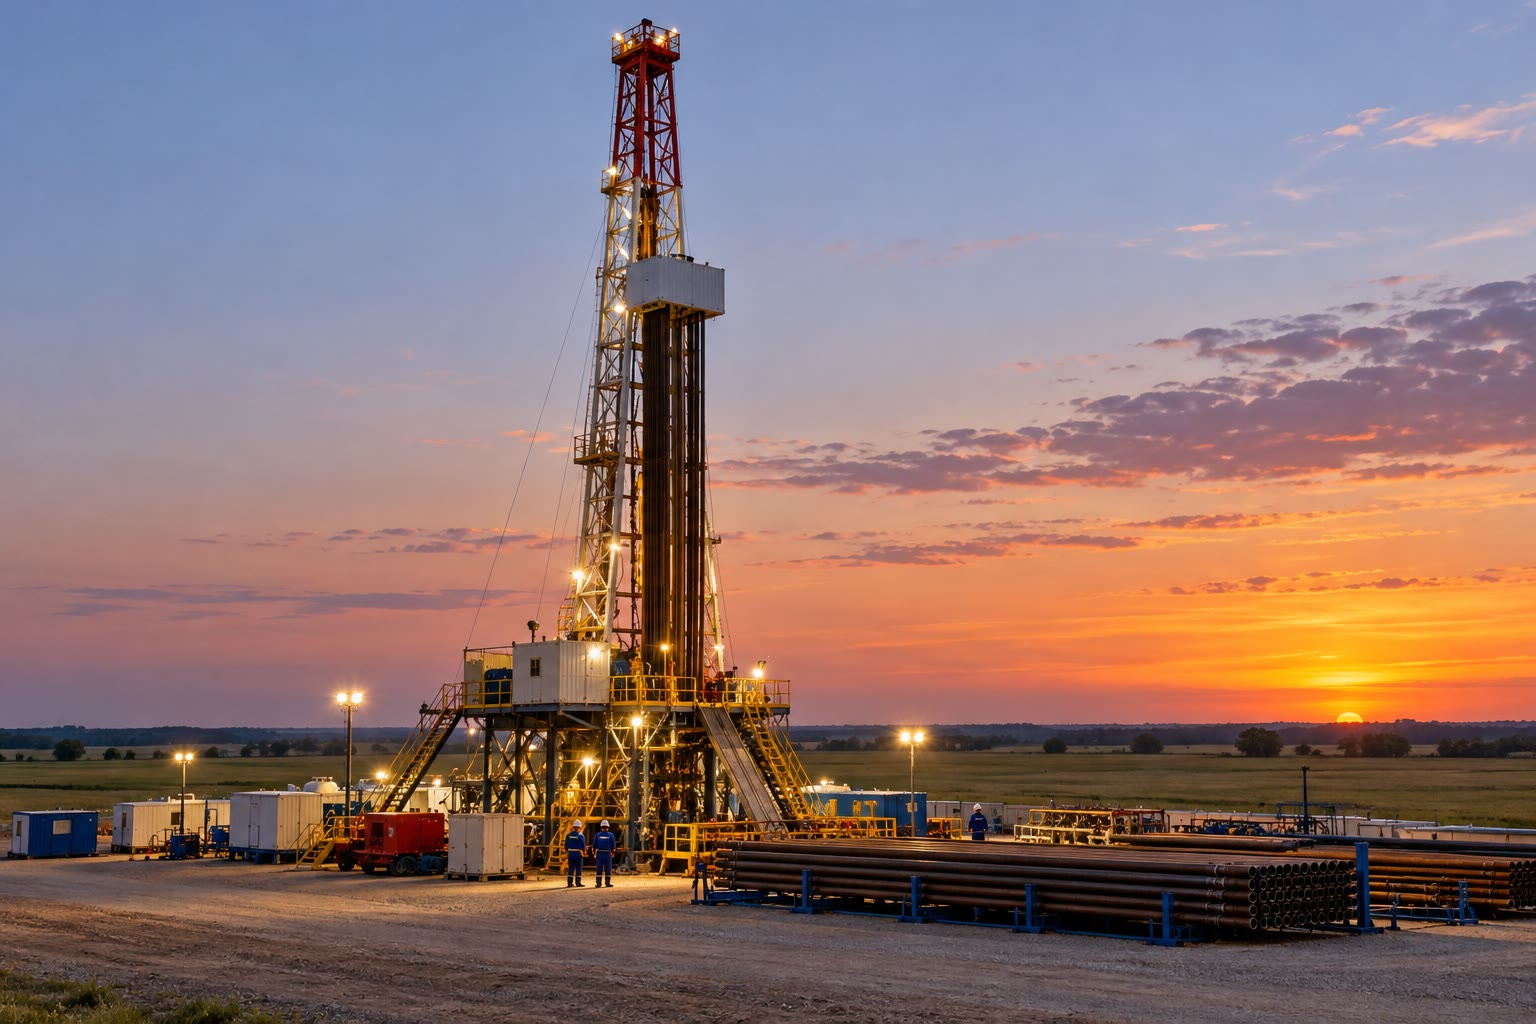
\includegraphics[width=0.3\linewidth]{images/book3/ai/b1-drilling-rig.jpg}\hfill
\begin{minipage}[b]{0.67\linewidth}
Quase tudo o que se sabe sobre o preenchimento profundo de uma bacia vem da busca por
petróleo, gás e água. Levantamentos de sísmica de reflexão fotografam suas camadas e suas
falhas ao longo de milhares de quilômetros quadrados; poços a amostram em um ponto. Um poço
devolve os cascalhos de rocha cortados pela broca, a intervalos testemunhos, e perfis
contínuos das propriedades físicas das rochas ao redor do furo, dos quais a porosidade é
lida metro a metro. As curvas porosidade--profundidade da \omterm{prop:b1:diagenesis-basins:athy}{lei de Athy}, e as histórias de
\omterm{def:b1:diagenesis-basins:subsidence}{subsidência} de bacias, foram construídas primeiro a partir de tais poços.
\end{minipage}

\smallskip
{\small Uma sonda de perfuração terrestre ao entardecer, com tubos empilhados em racks em
primeiro plano (ilustração de IA).}
\end{inthefield}
% ledger: sc80:north-sea

\section{Subsidência, acomodação e nível do mar}\label{sec:b1:diagenesis-basins:accommodation}

O sedimento só pode se acumular onde há espaço para ele abaixo do nível em que seria
removido. No mar esse nível fica perto do nível do mar, e o espaço é uma questão de dois
movimentos: o do fundo e o da superfície do mar.

\begin{definition}[Acomodação]\label{def:b1:diagenesis-basins:accommodation}
A \emph{acomodação}\index{acomodação} em um ponto de uma bacia é o espaço disponível para o
sedimento se acumular ali: a distância vertical do topo do sedimento ao nível do mar, o nível
de base da deposição marinha. A acomodação criada em um intervalo de tempo é o aumento da
distância de um datum preso ao embasamento até o nível do mar.
\end{definition}

\begin{definition}[Eustasia, nível relativo do mar]\label{def:b1:diagenesis-basins:eustasy}
\emph{Eustasia}\index{eustasia} é a mudança do nível do oceano mundial medida em relação a
uma referência fixa, o centro da Terra, causada por uma mudança no volume de água do oceano
ou no volume das bacias oceânicas; ela é a mesma em toda parte. O \emph{nível relativo do
mar}\index{nível relativo do mar} em um lugar é a altura da superfície do mar acima de um
datum preso ao embasamento ali; ele muda por eustasia e pelo movimento vertical do terreno.
\end{definition}

\begin{proposition}[O balanço de acomodação]\label{prop:b1:diagenesis-basins:budget}
Em um intervalo de tempo, seja $\Delta E$ a elevação eustática do nível do mar e $S$ o
afundamento do embasamento (ambos positivos para cima, no caso do mar, e para baixo, no caso
do fundo). A \omterm{def:b1:diagenesis-basins:accommodation}{acomodação} criada é
\[
  \Delta A = \Delta E + S ,
\]
e ela é repartida entre a espessura de sedimento acrescentada acima do datum,
$\Delta T$, e o aprofundamento da água, $\Delta W$:
$\Delta E + S = \Delta T + \Delta W$.
\end{proposition}

\begin{proof}
Meça as alturas a partir da referência fixa. Seja $e$ a altura da superfície do mar, $b$ a
do datum, $T$ a espessura de sedimento acima do datum, e $W$ a profundidade da água acima
do sedimento, de modo que $e = b + T + W$. O \omterm{def:b1:diagenesis-basins:eustasy}{nível relativo do mar} é $R = e - b = T + W$. No
intervalo, $\Delta e =
\Delta E$ e $\Delta b = -S$, logo $\Delta R = \Delta E + S$; e $\Delta R =
\Delta T + \Delta W$.
\end{proof}

Um fundo marinho mantido a profundidade constante ($\Delta W = 0$) é preenchido exatamente
tão depressa quanto a \omterm{def:b1:diagenesis-basins:accommodation}{acomodação} é criada; um que se torna mais raso é preenchido mais
depressa, e a linha de costa avança para o mar; um que se aprofunda fica subalimentado. $\Delta T$
é a mudança da espessura de toda a pilha acima do datum: ela conta o sedimento novo
depositado, menos o afinamento dos sedimentos mais antigos abaixo à medida que se compactam,
de modo que a própria \omterm{def:b1:diagenesis-basins:compaction}{compactação} abre espaço para mais sedimento (figura abaixo).

\begin{omfigure}
\begin{tikzpicture}[font=\footnotesize, >=Stealth]
\def\col#1#2#3#4#5{% x, datum, sediment top, sea, label
  \fill[lith granite] (#1,0.2) rectangle ++(1.4,#2-0.2);
  \fill[lith shale] (#1,#2) rectangle ++(1.4,#3-#2);
  \fill[lith sea] (#1,#3) rectangle ++(1.4,#4-#3);
  \draw[black!70] (#1,#2) -- ++(1.4,0);
  \draw[blue!60!black, thick] (#1-0.2,#4) -- ++(1.8,0);
  \node[anchor=north] at (#1+0.7,0.15) {#5};}
  \draw[black!60, dash dot] (-0.6,0.9) -- (8.6,0.9) node[anchor=west, align=left] {referência\\ fixa};
\col{0}{1.5}{3.0}{3.6}{tempo $t_1$}
\col{4.4}{1.0}{3.4}{3.9}{tempo $t_2$}
% eustasy
\draw[<->, omThm] (3.0,0.9) -- (3.0,3.6) node[midway, fill=white, inner sep=1pt] {$e_1$};
\draw[<->, omThm] (7.4,0.9) -- (7.4,3.9) node[midway, fill=white, inner sep=1pt] {$e_2$};
% subsidence of the datum
\draw[dashed, black!60] (1.4,1.5) -- (4.4,1.5);
\draw[->, thick] (4.2,1.5) -- (4.2,1.0) node[midway, anchor=east] {$S$};
% relative sea level
\draw[<->] (-0.35,1.5) -- (-0.35,3.6) node[midway, anchor=east] {$R_1$};
\draw[<->] (6.05,1.0) -- (6.05,3.9) node[midway, anchor=west] {$R_2$};
\node[anchor=west] at (1.5,2.25) {$T_1$};
\node[anchor=west] at (1.5,3.3) {$W_1$};
\node at (5.1,2.2) {$T_2$};
\node at (5.1,3.65) {$W_2$};
\node[anchor=south, align=center, blue!60!black] at (5.1,3.95) {nível do mar};
\node[anchor=west, align=left, font=\scriptsize] at (8.6,2.4) {$R = e - b = T + W$\\[2pt] $\Delta R = \Delta E + S$\\ $\phantom{\Delta R} = \Delta T + \Delta W$};
\end{tikzpicture}

{\small \omterm{def:b1:diagenesis-basins:accommodation}{Acomodação} em um lugar em dois tempos (esquemático). Entre $t_1$ e $t_2$ o nível do mar
sobe $\Delta E = e_2 - e_1$ acima da referência fixa e o embasamento afunda $S$: o \omterm{def:b1:diagenesis-basins:eustasy}{nível
relativo do mar} $R$ cresce $\Delta E + S$, a \omterm{def:b1:diagenesis-basins:accommodation}{acomodação} criada, que é repartida entre mais
sedimento ($T_2 > T_1$) e uma mudança da profundidade da água (aqui um leve raseamento,
$W_2 < W_1$).}
\label{fig:b1:diagenesis-basins:accommodation}
\end{omfigure}

Uma bacia não afunda só por sua \omterm{def:b1:diagenesis-basins:subsidence}{subsidência tectônica}: o sedimento que a preenche é uma carga,
e a \omterm{def:b1:layered-earth:lithosphere}{litosfera} afunda ainda mais sob ela.

\begin{proposition}[Carga sedimentar amplifica a subsidência]\label{prop:b1:diagenesis-basins:loading}
Em \omterm{def:b1:isostasy-gravity:isostasy}{isostasia} local (de Airy) sobre um \omterm{def:b1:layered-earth:layers}{manto} de densidade $\rho_m$, uma bacia cujo embasamento,
carregado apenas pela água de densidade $\rho_w$, ficaria na profundidade $Y$ abaixo do nível
do mar, contém, quando preenchida até o nível do mar com sedimento de densidade média
$\rho_s$, a espessura
\[
  h = Y\,\frac{\rho_m - \rho_w}{\rho_m - \rho_s}
\]
de sedimento. Em terra, preenchida até o nível dos arredores com ar acima, o fator é
$\rho_m/(\rho_m - \rho_s)$.
\end{proposition}

\begin{proof}
Compare as duas colunas com a mesma \omterm{def:b1:layered-earth:lithosphere}{litosfera}, de massa $M$ por unidade de área e espessura
$L$, até uma \omterm{def:b1:isostasy-gravity:isostasy}{profundidade de compensação} $z_c$ abaixo de ambas. A coluna carregada de água
tem $\rho_w Y + M + \rho_m(z_c - Y - L)$; a preenchida de sedimento,
$\rho_s h + M + \rho_m(z_c - h - L)$. Pela \cref{prop:b1:isostasy-gravity:equal-mass} as duas
massas são iguais, logo $\rho_w Y - \rho_m Y = \rho_s h - \rho_m h$, isto é, $h(\rho_m - \rho_s) =
Y(\rho_m - \rho_w)$. Com ar no lugar da água, $\rho_w$ é substituída por zero.
\end{proof}

Com $\rho_m = \qty{3300}{kg.m^{-3}}$, $\rho_w = \qty{1030}{kg.m^{-3}}$ e sedimento de densidade
média \qty{2300}{kg.m^{-3}}, o fator é $2270/1000 = \num{2.27}$: uma bacia cuja \omterm{def:b1:diagenesis-basins:subsidence}{subsidência
tectônica} abriria espaço para \qty{1}{km} de água contém \qty{2.27}{km} de sedimento. Em terra,
o fator seria $3300/1000 = \num{3.3}$. A densidade do preenchimento não é constante: ela cresce
à medida que o sedimento se compacta, e o fator com ela, de modo que transformar uma espessura
de sedimento em uma \omterm{def:b1:diagenesis-basins:subsidence}{subsidência tectônica} exige a \omterm{def:b1:diagenesis-basins:compaction}{descompactação} de cada camada, passo de tempo
a passo de tempo. Esse procedimento, o backstripping, pertence ao Livro~4.

O próprio nível do mar está longe de ser fixo. No Último Máximo Glacial, \omterm{def:b1:layered-earth:layers}{mantos} de gelo cobriam
grande parte da América do Norte e do norte da Europa, e a água presa neles tinha sido tirada do
oceano. Corrigidas pela resposta da Terra sólida às cargas variáveis de gelo e água, as
observações de antigas linhas de costa dão um nível do mar que caiu rapidamente cerca de
\qty{40}{m} há uns \num{30000} anos e depois lentamente, até \qty{134}{m} abaixo do atual, entre
\qtyrange{29}{21}{\ka}; o gelo apoiado sobre o leito tinha então cerca de \qty{52e6}{km^3} a mais
que hoje. O valor de \qty{125}{m} muitas vezes citado é menor porque geralmente não é corrigido
desses efeitos isostáticos. A deglaciação veio sobretudo entre cerca de \qty{16.5}{\ka} e
\qty{8.2}{\ka}, a uma média de \qty{12}{m} por mil anos, e a \qty{40}{mm} por ano ou mais entre
\qty{14.5}{\ka} e \qty{14.0}{\ka}.
% ledger: lambeck:lgm, lambeck:deglaciation

Níveis do mar mais baixos antigos são lidos a partir dos isótopos de oxigênio de foraminíferos
em testemunhos de mar profundo, que registram o volume de gelo em terra. Empilhando sete dessas
reconstruções nos últimos \num{430000} anos, e cinco nos últimos \num{800000}, as médias dos
erros de cada uma; reescalonado ao Holoceno e ao último rebaixamento glacial, o empilhamento
tem uma incerteza de \qtyrange{9}{12}{m} (figura abaixo). Ele mostra os ciclos glaciais como
um dente de serra: quedas lentas do nível do mar, cada uma terminada por uma subida rápida ---
cinco vezes nos últimos \num{800000} anos, uma subida de mais de \qty{100}{m} em menos de
\num{20000} anos. A \omterm{def:b1:diagenesis-basins:eustasy}{eustasia} nessa escala desloca a linha de costa para trás e para a frente
através das plataformas continentais.
% ledger: spratt:stack, data:b3-sealevel-stack

\begin{omfigure}
\begin{tikzpicture}[font=\footnotesize]
\begin{axis}[width=16cm, height=4.8cm, xmin=0, xmax=800, ymin=-150, ymax=40,
    x dir=reverse, xlabel={idade (milhares de anos antes do presente)}, xlabel style={yshift=2pt},
    ylabel={nível do mar (m)}, ytick={-150,-100,-50,0},
    title={(a) os últimos \num{800000} anos (cinco registros)}, title style={font=\footnotesize},
    axis on top]
  \addplot[draw=none, name path=hi] table[x=age, y=hi] {figdata/out/bachelor-1-sea_level-long.dat};
  \addplot[draw=none, name path=lo] table[x=age, y=lo] {figdata/out/bachelor-1-sea_level-long.dat};
  \addplot[omThm!25] fill between[of=hi and lo];
  \addplot[thin, omThm] table[x=age, y=sl] {figdata/out/bachelor-1-sea_level-long.dat};
  \draw[black!50, densely dotted] (axis cs:0,0) -- (axis cs:800,0);
\end{axis}
\end{tikzpicture}

\medskip
\begin{tikzpicture}[font=\footnotesize]
\begin{axis}[width=16cm, height=4.8cm,
    xmin=0, xmax=140, ymin=-160, ymax=40, x dir=reverse,
    xlabel={idade (milhares de anos antes do presente)}, ylabel={nível do mar (m)},
    ytick={-150,-100,-50,0},
    title={(b) os últimos \num{140000} anos (sete registros)}, title style={font=\footnotesize},
    axis on top]
  \addplot[draw=none, name path=hi] table[x=age, y=hi] {figdata/out/bachelor-1-sea_level-short.dat};
  \addplot[draw=none, name path=lo] table[x=age, y=lo] {figdata/out/bachelor-1-sea_level-short.dat};
  \addplot[omThm!25] fill between[of=hi and lo];
  \addplot[thick, omThm] table[x=age, y=sl] {figdata/out/bachelor-1-sea_level-short.dat};
  \draw[black!50, densely dotted] (axis cs:0,0) -- (axis cs:140,0);
  \addplot[only marks, mark=*, mark size=1.6pt, black] coordinates {(21,-134)};
  \draw[black!60, thin] (axis cs:21,-131) -- (axis cs:21,-46);
  \node[anchor=south, font=\scriptsize, fill=white, inner sep=1pt] at (axis cs:36,-46) {\qty{-134}{m} a \qty{21}{\ka} a partir de antigas linhas de costa (Lambeck et al.\ 2014)};
\end{axis}
\end{tikzpicture}

{\small Nível do mar global em relação a hoje, a partir do empilhamento de Spratt e Lisiecki
(2016): a primeira componente principal de cinco reconstruções a partir de testemunhos de mar
profundo ao longo de \num{800000} anos (a) e de sete ao longo dos últimos \num{140000} (b),
com sua faixa de um desvio padrão. O valor mais baixo do empilhamento, \qty{-130}{m} em
\qty{24}{\ka}, fica dentro dessa faixa dos \qty{-134}{m} encontrados a partir de antigas
linhas de costa (ponto); o último interglacial fica cerca de \qty{3}{m} acima de hoje, em
\qty{121}{\ka}. Dados: NOAA NCEI World Data Service for Paleoclimatology.}
\label{fig:b1:diagenesis-basins:sea-level}
\end{omfigure}
% computed in figdata/bachelor-1/sea_level.py; ledger: data:b3-sealevel-stack, spratt:stack, lambeck:lgm

Ao longo da vida de uma bacia essas oscilações são breves. Uma queda glacial de mais de
\qty{100}{m} em poucas dezenas de milhares de anos é rápida e grande comparada com a
\omterm{def:b1:diagenesis-basins:subsidence}{subsidência tectônica}, que soma um quilômetro ou mais apenas ao longo de dezenas de milhões de
anos; mas as oscilações glaciais permanecem dentro de uma faixa de cerca de \qty{150}{m}, de
modo que, no preenchimento espesso de uma bacia, a \omterm{def:b1:diagenesis-basins:subsidence}{subsidência} faz a maior parte do espaço, e a
\omterm{def:b1:diagenesis-basins:eustasy}{eustasia} define o ritmo de suas camadas.
% ledger: data:b3-sealevel-stack, sc80:north-sea

\section{Exercícios}

\begin{exercise}[$\star$]\label{exo:b1:diagenesis-basins:1}
Com os parâmetros da \cref{tab:b1:diagenesis-basins:athy}, calcule a porosidade do arenito e
do folhelho a \qty{2000}{m}. A que profundidade a porosidade de cada um caiu até a metade de
seu valor superficial?
% ledger: pybacktrack:compaction
\end{exercise}

\begin{exercise}[$\star$]\label{exo:b1:diagenesis-basins:2}
Durante um intervalo de tempo, o nível do mar sobe \qty{30}{m} por \omterm{def:b1:diagenesis-basins:eustasy}{eustasia}, o embasamento de
uma plataforma afunda \qty{50}{m}, e \qty{60}{m} de sedimento se acrescentam acima de um datum
sobre o embasamento. Com \cref{prop:b1:diagenesis-basins:budget}, calcule a \omterm{def:b1:diagenesis-basins:accommodation}{acomodação} criada
e a mudança da profundidade da água. A plataforma aprofunda-se ou raseia-se?
\end{exercise}

\begin{exercise}[$\star$]\label{exo:b1:diagenesis-basins:3}
A \omterm{def:b1:diagenesis-basins:subsidence}{subsidência tectônica} de uma bacia abriria espaço para \qty{1.0}{km} de água. Com
$\rho_m = \qty{3300}{kg.m^{-3}}$ e $\rho_w = \qty{1030}{kg.m^{-3}}$, qual é a espessura do
sedimento que a preenche até o nível do mar se sua densidade média for
\qty{2300}{kg.m^{-3}}? \qty{2500}{kg.m^{-3}}? Por que um preenchimento mais denso dá um mais
espesso?
\end{exercise}

\begin{exercise}[$\star$]\label{exo:b1:diagenesis-basins:4}
A calcita tem massa molar \qty{100.09}{g.mol^{-1}} e densidade \qty{2.71}{g.cm^{-3}}; a
dolomita, \qty{184.40}{g.mol^{-1}} e \qty{2.84}{g.cm^{-3}}. (a)~Calcule o volume molar de cada
uma. (b)~Em que fração muda o volume do sólido quando dois mols de calcita se tornam um mol de
dolomita? (c)~Um calcário de porosidade \num{0.10} é dolomitizado mol por mol sem mudança de
seu volume externo. Qual é sua nova porosidade?
% ledger: hom:calcite, webmineral:others
\end{exercise}

\begin{exercise}[$\star\star$]\label{exo:b1:diagenesis-basins:5}
Um folhelho ocupa o topo de \qty{1000}{m} de uma bacia. (a)~Calcule sua espessura sólida e sua
porosidade média. (b)~Ele é soterrado até que seu topo fique a \qty{2000}{m}. Usando
\cref{met:b1:diagenesis-basins:decompaction} com o topo deslocado para baixo em vez de para
cima, encontre sua nova espessura e sua porosidade média. (c)~Quanta água cada metro quadrado
do folhelho expeliu?
% ledger: pybacktrack:compaction
\end{exercise}

\begin{exercise}[$\star\star$]\label{exo:b1:diagenesis-basins:6}
Um arenito está entre \qty{2500}{m} e \qty{2800}{m}. (a)~Calcule sua espessura sólida.
(b)~Descompacte-o até a superfície com \cref{met:b1:diagenesis-basins:decompaction},
anotando cada passo de Newton a partir de $b_0 = \qty{300}{m}$. (c)~Por qual fator o
soterramento o afinou?
% ledger: pybacktrack:compaction
\end{exercise}

\begin{exercise}[$\star\star$]\label{exo:b1:diagenesis-basins:7}
No Último Máximo Glacial o gelo apoiado sobre o leito tinha cerca de \qty{52e6}{km^3} a mais
que hoje. Tome a densidade do gelo \qty{916.7}{kg.m^{-3}}, a da água de degelo
\qty{1000}{kg.m^{-3}}, e a área do oceano de hoje \qty{361.84e6}{km^2}. (a)~Que queda do nível
do mar esse gelo representa? (b)~Compare com os \qty{134}{m} encontrados a partir de antigas
linhas de costa. (c)~Que área oceânica daria exatamente \qty{134}{m}, e por que o oceano
glacial era menor?
% ledger: lambeck:lgm, iapws:ice-density, charette:ocean-volume
\end{exercise}

\begin{exercise}[$\star\star$]\label{exo:b1:diagenesis-basins:8}
O empilhamento do nível do mar dá \qty{-98.1}{m} em \qty{16}{\ka} e \qty{-9.1}{m} em
\qty{8}{\ka}. (a)~Calcule a taxa média de subida, em metros por mil anos, e compare-a com os
\qty{12}{m} por mil anos encontrados a partir de antigas linhas de costa para a principal
deglaciação. (b)~Entre \qty{14.5}{\ka} e \qty{14.0}{\ka} o nível do mar subiu a \qty{40}{mm}
por ano ou mais. Quantas vezes a média isso é, e quanto o nível do mar subiu nesses quinhentos
anos?
% ledger: data:b3-sealevel-stack, lambeck:deglaciation
\end{exercise}

\begin{exercise}[$\star\star$]\label{exo:b1:diagenesis-basins:9}
Uma plataforma está sob \qty{20}{m} de água. Seu embasamento afunda a \qty{50}{m} por milhão
de anos. (a)~Em dois milhões de anos o nível do mar cai \qty{40}{m} por \omterm{def:b1:diagenesis-basins:eustasy}{eustasia} enquanto a
profundidade da água permanece a mesma. Quanta \omterm{def:b1:diagenesis-basins:accommodation}{acomodação} é criada, e quanto sedimento é
acrescentado? (b)~Em seguida o nível do mar cai \qty{120}{m} em \num{20000} anos, no início de
uma glaciação, e nenhum sedimento é acrescentado. A que altura acima do nível do mar fica o
antigo fundo marinho no fim?
\end{exercise}

\begin{exercise}[$\star\star\star$]\label{exo:b1:diagenesis-basins:10}
(a)~Mostre que uma camada de espessura $h$ à profundidade $z$, fina comparada com o
comprimento de decaimento $\lambda$, tem a espessura $h_0 \approx h\,(1 - \varphi(z))/(1 -
\varphi_0)$ quando restaurada à superfície. (b)~Aplique-a a \qty{10}{m} de folhelho a
\qty{3000}{m}, e compare com a \omterm{def:b1:diagenesis-basins:compaction}{descompactação} exata, \qty{23.1}{m}. (c)~Por que a aproximação
é um pouco grande demais?
% ledger: pybacktrack:compaction
\end{exercise}

\begin{exercise}[$\star\star\star$]\label{exo:b1:diagenesis-basins:11}
Uma bacia é preenchida até o nível do mar por \qty{3000}{m} de folhelho, compactado pela \omterm{prop:b1:diagenesis-basins:athy}{lei
de Athy}, com os poros cheios de água de densidade \qty{1030}{kg.m^{-3}}. (a)~Calcule a
porosidade média e a densidade média do preenchimento. (b)~Com
\cref{prop:b1:diagenesis-basins:loading} e $\rho_m =
\qty{3300}{kg.m^{-3}}$, calcule o fator de carga e a \omterm{def:b1:diagenesis-basins:subsidence}{subsidência} com água que o preenchimento
representa. (c)~Por que tomar a densidade dos grãos, \qty{2700}{kg.m^{-3}}, daria um fator muito
maior, e por que isso estaria errado?
% ledger: pybacktrack:compaction
\end{exercise}

\begin{exercise}[$\star\star\star$]\label{exo:b1:diagenesis-basins:12}
Um metro cúbico de calcário de porosidade \num{0.10} deve ser dolomitizado completamente, mol
por mol. A água do mar contém \qty{35.165}{g} de sal por quilograma, dos quais a fração em
massa \num{0.0365} é magnésio (\qty{24.305}{g.mol^{-1}}). (a)~Quantos mols de calcita há no
cubo (volume molar de \cref{exo:b1:diagenesis-basins:4})? (b)~Quantos mols de magnésio a
reação precisa? (c)~Que massa e que volume de água do mar (\qty{1030}{kg.m^{-3}}) devem fluir
pelo cubo se ele entregar todo o seu magnésio? (d)~O que a resposta diz sobre onde a dolomita
se forma?
% ledger: teos10:reference-composition, teos10:reference-salinity, hom:calcite
\end{exercise}

\section{Problema: descompactando o preenchimento de uma bacia}

\begin{problem}[{Problema de fim de semana --- quão espessos eram os sedimentos de um poço
quando foram depositados, e como o espaço para eles foi criado}]
\label{pb:b1:diagenesis-basins:1}
% values: calc/ch23.py; the well, its units, ages and the eustatic changes are invented
Um poço perfurado em uma planície costeira, ao nível do mar, atravessa três unidades antes
de atingir o embasamento a \qty{3200}{m}:
\begin{center}
\begin{tabular}{llll}
\hline
unidade & litologia & profundidade hoje (m) & tempo de deposição \\
\hline
1 & arenito & 0--800     & \qtyrange{15}{0}{\Ma} \\
2 & folhelho & 800--2600  & \qtyrange{55}{15}{\Ma} \\
3 & giz      & 2600--3200 & \qtyrange{75}{55}{\Ma} \\
\hline
\end{tabular}
\end{center}
Tome os parâmetros da \cref{tab:b1:diagenesis-basins:athy}, água de poros de densidade
\qty{1030}{kg.m^{-3}}, $g = \qty{9.81}{m.s^{-2}}$, e suponha que cada unidade foi compactada
pela \omterm{prop:b1:diagenesis-basins:athy}{lei de Athy}, com sua água livre para escapar, durante toda a sua história. Microfósseis
mostram que a água era rasa, e de mesma profundidade, no início e no fim de cada intervalo.

\medskip
\noindent\textbf{Parte I --- A coluna hoje.}
\begin{enumerate}
  \item Calcule a porosidade no topo e na base de cada unidade.
  \item Calcule a porosidade média de cada unidade.
  \item Quanta água cada unidade contém sob um metro quadrado?
  \item Calcule a densidade aparente de cada unidade, saturada de água, e a densidade média
        de toda a coluna.
  \item Calcule as pressões litostática e hidrostática na base da coluna, e a \omterm{def:b1:stress-strain-rheology:lithostatic}{tensão efetiva}
        ali.
  \item A que profundidade as porosidades do arenito e do folhelho são iguais? Qual é a mais
        porosa abaixo dela?
\end{enumerate}

\noindent\textbf{Parte II --- Os grãos.}
\begin{enumerate}[resume]
  \item Calcule a espessura sólida de cada unidade.
  \item Qual é a espessura sólida de toda a coluna, e que fração da coluna de hoje é água?
  \item Calcule, para cada unidade, a taxa de acumulação de grãos, em metros de sólido por
        milhão de anos.
  \item Qual unidade teve o suprimento de grãos mais rápido? A mais lenta?
\end{enumerate}

\noindent\textbf{Parte III --- As unidades como foram depositadas.}
\begin{enumerate}[resume]
  \item Qual era a espessura do arenito quando foi depositado? Por que nenhum cálculo é
        necessário?
  \item Descompacte o folhelho até a superfície: qual era sua espessura a \qty{15}{\Ma}, quando
        sua deposição tinha acabado de terminar?
  \item Descompacte o giz até a superfície: qual era sua espessura a \qty{55}{\Ma}?
  \item Qual era a espessura do giz a \qty{15}{\Ma}, soterrado sob o folhelho da questão
        anterior?
  \item Qual era a espessura de toda a coluna acima do embasamento a \qty{55}{\Ma} e a
        \qty{15}{\Ma}?
  \item Calcule a taxa de sedimentação de cada unidade a partir de sua espessura hoje, e a
        partir de sua espessura na deposição. Qual delas é a significativa?
  \item Em que fração o folhelho afinou desde \qty{15}{\Ma}?
\end{enumerate}

\noindent\textbf{Parte IV --- Fazendo espaço.}
\begin{enumerate}[resume]
  \item Tome o topo do embasamento como datum. Com \cref{prop:b1:diagenesis-basins:budget},
        calcule a \omterm{def:b1:diagenesis-basins:accommodation}{acomodação} criada de \qtyrange{75}{55}{\Ma}, de \qtyrange{55}{15}{\Ma} e de
        \qty{15}{\Ma} até hoje.
  \item Uma curva eustática para a região dá o nível do mar \qty{60}{m} mais alto a
        \qty{55}{\Ma} do que a \qty{15}{\Ma}, e \qty{30}{m} mais alto a \qty{15}{\Ma} do que hoje
        (valores assumidos). Calcule a \omterm{def:b1:diagenesis-basins:subsidence}{subsidência} do embasamento nos dois últimos intervalos.
  \item Calcule a taxa média de \omterm{def:b1:diagenesis-basins:subsidence}{subsidência} em cada um, em metros por milhão de anos.
  \item Que parte da \omterm{def:b1:diagenesis-basins:subsidence}{subsidência} a \omterm{def:b1:diagenesis-basins:eustasy}{eustasia} teve de compor em cada intervalo? A \omterm{def:b1:diagenesis-basins:eustasy}{eustasia}
        ajudou ou atrapalhou o preenchimento da bacia?
  \item Da \omterm{def:b1:diagenesis-basins:accommodation}{acomodação} preenchida desde \qty{15}{\Ma}, quanta foi criada pela \omterm{def:b1:diagenesis-basins:compaction}{compactação} do
        folhelho e do giz abaixo?
  \item Por que a \omterm{def:b1:diagenesis-basins:subsidence}{subsidência} do embasamento não pode ser lida a partir da espessura da coluna
        hoje?
  \item Qual era a espessura da unidade de folhelho quando foi depositada?
\end{enumerate}
\end{problem}
